\documentclass{uvamscse}
\input{program-listings}
\usepackage{verbatim}
\usepackage{hyperref}
\usepackage{algorithm}
\usepackage{algorithmic}
\usepackage{graphicx}
\graphicspath{ {./graphs/} }
\newcommand{\cmd}[1]{\texttt{$\backslash$#1}}
\sloppy

\title{Dead Code Detection \\ on Strict ECMAScript 6 Projects}

\author{Alberto Martinez de Murga Ramirez}
\authemail{alberto@threkk.com}

\supervisor{Vadim Zaytsev, Universiteit Twente}

\abstract{
JavaScript is a dynamic scripting language that has surged in popularity and ubiquity in the recent years. Due to the rapid progress of the language and its ecosystem, it is common to find out projects that have evolved rapidly as the language. This leads to the proliferation of dead code is such projects. We research how we can fight dead code in JavaScript projects using the version 6 of ECMAScript by performing static analysis based on call-graphs, concretely a new type of call-graph described in the document too. After identifying the issues regarding static analysis in this context, the reasons and mitigation, we describe an an algorithm to detect dead code at different levels of the project: dependencies, modules and statements. After testing the proof of concept against different projects, we find that results show that it is a feasible approach but with a high dependency on the quality of the call-graph. 
}

\begin{document}
\maketitle
%%%%%%%%%%%%%%%%%%%%%%%%%%%%%%%%%%%%%%%%%%%%%%%%%%%%%%%%%%%%%%%%%%%%%%%%%%%%%%%%
\chapter{Problem statement and motivation}
Web applications are one of the most common software products built: from simple portfolios to complex corporate systems. With over 1.5 billion websites around, the development and maintenance of a wide range of websites is not a trivial task and it has evolved quickly in the last years.

Traditionally web page consisted of a group of HTML files. Later some scripts in languages like Perl or PHP were added. Nowadays, the complexity has increased, with the addition of different types of databases, several server languages, layers of abstraction and more evolved front end techniques.

The front end part of web applications has evolved especially fast in the latest years with the appearance of complex frameworks like React\footnote{\url{https://reactjs.org/}}, Angular\footnote{\url{https://angular.io/}} or Vue\footnote{\url{https://vuejs.org/}}. These frameworks share the same characteristics: designed for complex front end application, usage of advanced features of JavaScript with transpilation, fast evolution and focusing on performance and dynamic content.

Current web applications and web based systems are considered \textit{E}-programs under Lehman's classification system \cite{10.1109/PROC.1980.11805}. \textit{E}-programs are those evolving programs which are applied to activities which interact with the environment. \textit{E}-programs must add features over time to keep users satisfied. As \textit{E}-programs evolve, they become more complex. The increase of complexity implies a declination of quality without maintenance. Because the system is continuously growing, the system becomes more complicated to maintain.

The fast cycles (for instance, React has accrued 17 major versions\footnote{Until the current month of August 2021} since 2013) lead to many breaking changes being applied to existing or on development projects. These constant changes, in combination with the changes or re-implementation of features, leave behind a trail of code which is not used or executed any more in the project. The purpose of this code has been forgotten and it is still there because it was the dependency of a dependency and no one remembers exactly how it got there. We will call this type of old and useless code \textbf{dead code}.

A dead code fragment is a fragment of source code of a program which is never used in other part of the program. This section is not executed, stripped internally by the compiler; or not used, wasting computation time and resources. This code is still present in the project and it needs to be maintained even if it is not used. It consumes developers time and resources, making the project bigger and more complex than it should be. Bigger projects are harder to maintain and develop. Identifying and potentially removing this type of code will decrease the size of it and make the maintenance and development easier and simpler.

Dead code then increases the size of the software, making it bigger and harder to maintain based on Lehman's laws mentioned. By removing dead code, it contributes to the maintenance by keeping the program size in check.

The aim of this project is to develop a tool which identifies this type of code. There are some existing tools which already transpiles source code like \textit{Google Closure}. However, these tools are aimed to produce minified code for production deployment rather than to increase developer productivity. The desired tool is developer focused and it would be able to identify which portions of code and dependencies are not allegedly used any more and can be safely removed.

Given the big scope that this project it could cover, we are focusing on modern web applications. This means that we are aiming to detect dead code in strict ECMAScript version 6.

The \textbf{contributions} of this thesis are the following:
\begin{itemize}
    \item Description of the current state of dead code analysis in JavaScript.
    \item Proposal for a new approach in detecting dead code, including a new technique to generate call graphs.
    \item Proof of concept of the approach.
    \item Analysis of a set of open source projects with the tool.
\end{itemize}

\chapter{Background and context}
We are centring our research on detecting dead code in JavaScript projects using ECMAScript version 6. This choice is not arbitrary, as it is the considered the current baseline of modern JavaScript that can be executed in most of the platforms. JavaScript is a language that syntactically looks like Java or C, but it has many differences with them, which they can be attributed to its evolution as a language. These differences give the language some properties that influence the search of dead code, which itself is already a complicated task. In this chapter, we will review the history and characteristics of the JavaScript language, and we will get an overview of the meaning of searching for dead code.
\section{The JavaScript language}
%% In this section, I want to expose how complicated is the JavaScript ecosystem to analyse, specially in order to do static analysis as it is totally opposite to its dynamic nature. Therefore, the possibilities of static analysis are reduced.
\subsection{History of the language}
The JavaScript language was created in 1995 by Brendan Eich as part of the version 2.0 of the Netscape browser (currently abandoned). The original purpose was to make a small ``glue language" that was easy to use by designers and part-time programmers to assemble components like images, where the code could be written in a familiar syntax in the HTML files.

The language originally ran on the Netscape browser, with Microsoft reverse engineering its own scripting technologies for the browser, named VBScript and JScript. In 1996, Netscape submitted the JavaScript specification to the European Computer Manufacturers Association (\textbf{ECMA}) with the intention that other browsers could implement the JavaScript language. This lead to the release of ECMAScript language specification in 1997. Soon after that, the version 2 was released in 1998 and the version 3 in 1999.

Initially, Microsoft had no intention of implementing JavaScript on Internet Explorer. The other major browser at that time, had its own versions of the scripting language for the front end, which became a big problem for developers aiming to support all the browsers on their pages. Therefore, the work on the version 4 of ECMAScript started in 2003 without Microsoft support.

The development on the version 4 was affected by the different positions about how ambitious the changes should be and possible backwards compatibility issues~\cite{IEBrokenWeb}. On one side, Brendan Eich, Mozilla, Macromedia, and Adobe joined to the efforts of the development of ECMAScript 4. On the other side, Microsoft, Yahoo and Google opposed ECMAScript 4. ECMAScript 4 was never completed and, instead, ECMAScript 3.1 was released as a strict subset of ECMAScript 4. Finally, in July 2008 both sides gathered in Oslo to reach an agreement on the rename of ECMAScript 3.1 into ECMAScript 5 and the collaboration on a common line of development with all the actors~\cite{TC39Oslo}.

ECMAScript 5 was released in 2009, followed by a version 5.1 in 2010 to fully align with the ISO/IEC 16262. After this version, subsequent versions have been released every year with substantial improvements and changes to the language: ECMAScript 6 (2015), ECMAScript 7 (2016) and ECMAScript 8 (2017).

The language had also several implementations server side. Netscape introduced an implementation for the language into Netscape Enterprise Server in 1995 and Microsoft supported JScript in ASP and .NET pages since 1996. In 2009, Node.js was released based on the JavaScript engine V8 of the Chrome browser. This is currently the most popular and widely used implementation of JavaScript server side~\cite{JSHisMDN,keith2011dom}.

In the latest years, its ubiquity and popularity has extended its usage, making JavaScript even more popular. Nowadays is possible to use JavaScript for front end, back end (\textit{Node.js}), databases (\textit{MongoDB}, \textit{DynamoDB}), videogames (\textit{UnityScript}), operative systems (\textit{JavaScript for Automation}, \textit{WinJS}), mobile phones (\textit{React Native}, \textit{KaiOS}).

\subsection{Characteristics of the language}
JavaScript was born as a scripting language, as we saw above. As a scripting language, it shares some characteristics with other scripting languages like Python or Ruby, although JavaScript still has some characteristics which are exclusive of it.

JavaScript is a \textbf{loosely typed} or dynamically typed language which also performs several types of automatic type conversions between variable types. It supports seven different types: \texttt{String}, \texttt{Number}, \texttt{Boolean}, \texttt{BigInt}, \texttt{Symbol}, \texttt{null} and \texttt{undefined}. All these types are known as \textbf{primitive types}, being the additional type \texttt{Object} the only data structure. It is important to notice that both \texttt{Array} and \texttt{Function} are not data structures but sub-types of \texttt{Object}. All variables that are not declared or declared without a value have automatically the type and value \texttt{undefined} which itself is the lack of value. Once declared, the variable can have any of the types mentioned, including \texttt{null}, the type and value which indicates the conscious nonexistent or invalid value. It is important to notice as well that \texttt{undefined} and \texttt{null}, although they look similar, they are not the same~\cite{MDNTypes,MDNNull,MDNUndefined}.

JavaScript can change the type of the variables depending or the context in which it is used at any moment. These type conversions are not consistent, leading to common errors. For instance, an empty array (\texttt{[]}) evaluates to \texttt{true} when used in an \textit{if-statement}, but an empty string (\texttt{""}) evaluates to \texttt{false} in the \textit{if-statement}. In other example, the operation \texttt{"1" + 1}, being the first operand the string representation of the number one and the second the number one, will return the string \texttt{"11"}, result of evaluating the second operand to \texttt{string} and concatenating both of them. However, the same operation but changing the operand to minus (\texttt{"1"-1}) will return zero, in this  case evaluating the first operand to \texttt{number}~\cite{FlanaganDavid2011J:td}.

JavaScript is a \textbf{prototype based language}. Although it might look familiar for developers who are used to class based languages like Java or C++, it is dynamic and their \texttt{class} keyword is no more than syntactic sugar. Any object can inherit methods and properties from other object by setting their prototype to another object. The prototype is always defined, creating a chain of objects until reaching the top of the chain, which is the \texttt{Object} prototype, or \texttt{null}. When a property is accessed, JavaScript looks for it in the current object, and if it does not find it, it goes up into the prototype chain until the property is found or the chain ends~\cite{MDNProtoType}. This means that if any object changes its properties or prototypes, the changes are transmitted along the chain, being uncertain at some point of the execution if an object still holds certain properties.

This also relates with the \textbf{dynamic nature of JavaScript}, which allows to change the code on run time. It can change its properties and prototypes on run time. If you try to set an nonexistent property of an object on run time, instead of throwing an exception, JavaScript will create it on run time, or if you try to read it, it will return \texttt{undefined}. JavaScript is also able to execute code dynamically from a string using the function \texttt{eval}, hoist variables and function names altering the execution order, and introduce new scopes for variables and functions on run time~\cite{SunKwangwon2017AoJP}. The context is not an exception, it is possible to change the context of a function by using different functions like \texttt{call}, \texttt{bind}, or \texttt{apply}. This functions allow to change the resolution of the symbols of the function by using a different provided context instead of the default one. This is heavily used in libraries. Function arity is also dynamic. A function can have a defined amount of parameters, but when the function is called, it accepts an arbitrary number of arguments. If there are less than the defined ones, the remaining are initialised as \texttt{undefined}; if there are more, they are ignored.

JavaScript is also heavily influenced by functional paradigm. It uses anonymous functions and callbacks extensively, and until the ECMAScript version 6 it did not support any type of module system, being necessary the usage of workarounds and patterns to achieve similar effects. This makes the creation of call graph constructions complicated compared to other languages~\cite{SunKwangwon2017AoJP}.

\section{Dead code overview}
Dead code is code which is never used or reachable. It is not harmful by itself since it does nothing but it is considered a ``bad smell" in the code. A ``bad smell" is a symptom of bad implementation or design that corresponds to a deeper problem in the system~\cite{FowlerSmells}.

Dead code is quite common, in some cases like in \cite{DeadCodePHP} it can be around 30\% of the code base. On \cite{ICSE-2012-EderJJHVP} they found that about 25\% of the methods defined were not used for two years, but the support of these features implied 50\% of the effort invested in maintenance. Similar results were obtained by \cite{ICSE-2012-EderJJHVP}. They monitored the maintenance actions of an industrially hosted business information system for over two years and found that 25\% of all methods was not used, but only 7.6\% of the maintenance actions were spent on those concrete methods. However, 48\% of the maintenance actions that were performed on the unused parts of the system were also unnecessary.

The dead code appear in several ways. It can be created already dead, when developers create functions, methods and modules that they plan to use but they end up not using. This is related to breaking the \textbf{YAGNI} (\textit{You aren't gonna need it}) principle of extreme programming, when developers create a functionality that is not necessary~\cite{RonJeffriesXP}. It can also turn dead during the software evolution, for instance, by developers who do not remove outdated code. This gets worse if the code base is inherited from a previous team \cite{MultistudyDeadCode}.

Dead code is perceived by developers as an obstacle to understand and modify source code, especially when it is unfamiliar \cite{MultistudyDeadCode}, although it is not one of their main concerns, ranking 10\textsuperscript{th} out of 13 code smells at \cite{6671299}.
\subsection{State of the art on dead code detection}

As we stated before, dead code is a common issue in all types of projects and languages. There have been several attempts to find and remove dead code in different contexts using different techniques. Given that our aim is to find the concrete pieces of code, the analysis will focus on the research done in the detection of dead code.

In \cite{DeadCodePHP}, the research aims to the same objective but targeting the PHP language. Their approach consists of a dynamic analysis to determine the file coverage and frequency of each file. Unused files are targeted as potentially dead. This approach was successful in the given context, allowing to remove more than 60\% of the files in some projects.

% XQuery Paper
A different approach is used in \cite{DeadCodeXQuery}, based in static analysis in order to detect dead code in XQuery programs by checking if the rules described in the program are meaningful to the schema which defines the input of it. The software produced was able to identify and strip the dead code from XQuery programs.

% Java call graphs paper
In the Java language, we can find in \cite{JavaDeadCode} a proposal to detect unreachable code which outperforms other solutions on correctness, completeness, and accuracy. Unreachable code a sub type of dead code. It is code which is never reached by any means. The approach is based on building a call graph of methods and use it to find the nodes which are not reachable from the main method.

There have been previous attempts to detect dead code in JavaScript projects. In \cite{JNose} it is presented a metric-based approach combines static and dynamic analysis by setting a combination of metrics and thresholds like the amount of lines of code or number of properties to detect smells in client-side code. In order to detect unused/dead code, they recognise how challenging it is to perform static analysis on JavaScript code due to its dynamic nature, so their criteria is to mark as dead all those functions which execution counter is zero after executing the web application. 

Targeting EcmaScript 5 front end projects, \cite{ieee_s8330226} presents \textit{Lacuna} which uses a combination of dynamic and static analysis to build execution generated flow graphs and \textit{WALA} based call graphs that are combined into a single call function graph. It considers dead code any node of the graph which is not reachable from the global node. 

% Not all the studies are based on concrete languages. Other studies refer to general approaches to treat dead code that can be applied to different contexts.
In \cite{KnoopJens1994Pdce}, they distinguish between dead code and partially dead code. Partially dead code is dead code that is only dead in certain branches of execution. The authors determine that is impossible to remove the partially dead code without changing the branching structure of the program or impairing some program executions. The proposed algorithm implies a series of assignment shrinking by moving or elimination variables assignments and the removal of new dead branches that after several iterations produces an equivalent program without partial dead code.

\subsection{Analysis of JavaScript projects}
The research on the JavaScript projects is divided in several trends of which static analysis is the most relevant to the current context. The most researched topic has been the static analysis of JavaScript projects, but the dynamic features and the web execution environments make it very challenging. To lessen the imprecision of static analysis, dynamic analysis complements it.\cite{SunKwangwon2017AoJP}

% Challenges of static analysis.
The challenges of static analysis are related to its dynamic nature. Types can change during run time, code can be generated and executed during the execution, and objects can modify their properties. These characteristics make static analysis imprecise and difficult.

As summarised in \cite{FeldthausAsger2013Ecoa}, variables have no static types and may hold several values of different types during execution. Object do not have fixed properties, and they can be created on run time by assigning a value to an undefined property. Any property can also change its value or being deleted at any moment. Functions are first-class objects, and they can be passed as arguments, stored as object properties or as a variable, and even have properties themselves. By reassigning the variable name, they can also stop being functions at any moment. Functions also can have a variable amount of arguments and it is possible to call a function with more or less parameters than expected in its definition. Dynamic properties also allow accessing to properties by computed names.

If the execution happens to be in the browser, the DOM (\textit{Document Object Model}), browser events, and user interactions increase the complexity of the analysis as well as a huge amount of functions are added to the global space. If not properly isolated by the developer, other libraries will pollute the global space too. The dynamic analysis helps to overcome some of these issues by executing the DOM APIs and other user related events and using the output of the executions based on the events for the analysis.

Most of the approaches to static analysis in JavaScript imply the creation of call graphs. A call graph is a control flow graph which represent the calling relationships between different functions and variables of a program \cite{FeldthausAsger2013Ecoa}. Call graphs are essential to build static analysis tools.

% Examples of the papers we have in static analysis and call graphs papers.
There have been several attempts of performing static analysis on JavaScript both from an academic and industry perspectives. From the academic perspective we can stand out \textit{TAJS}, \textit{SAFE}, and \textit{JSAI}. There has been other attempts to create call graphs using events instead of functions \cite{MadsenMagnus2015Saoe}, which are really helpful to detect dead listeners and dead emits.

\textit{TAJS} \cite{tajs2009} is one attempt to perform type analysis in JavaScript by using flow graphs. The flow graphs model the statements into nodes depending on their purpose and joins them by edges depending if they are intra-procedural flows, exceptions handling or function calls. The types are calculated by applying lattice and transfer functions. The result is a flow-sensitive type analyser which detect typical errors like calling non-functions as if they were functions.

\textit{SAFE} \cite{lee2012safe} presents a formal specification and implementation of a scalable analysis framework for ECMAScript 5 targeted to the JavaScript research community. It includes its own parser, formal description and implementation of the version 5 of ECMAScript. This tools is later used to implement tools like code coverage and clone detectors. The follow up work includes extensions like \textit{SAFEwapi} \cite{safewapi} or \textit{SAFEwapp} \cite{safewebapp} which detect miss usage of WebAPI's due to different vendor implementations and a general web application analysis tool.

\textit{JSAI} \cite{JSAI} is similar to TJAS in its purpose of creating an extensible static type analysis tool. It bases the analysis in formally specified concrete and abstract JavaScript semantics, and it has been tested with several JavaScript engines.

% Estree (Acorn, Esprima), Babylon, WALA
Some other analysers have been developed outside academic circles. The most important project in this area is the ESTree specification~\cite{ESTree}, which has been used in analysers like Espree, Acorn, Esprima, Babylon, or WALA.

The ESTree specification\cite{ESTree} was created by David Herman, a Mozilla engineer, while documenting the output of an API that exposed the \textit{SpiderMokey} JavaScript parser. The format exposed in that document became standard for tools that manipulate JavaScript source code. Currently is maintained and developed by group with members of the main parser tools that implement the specification. The specification aims to be backwards compatible, context independent, avoid duplicated information, and extensible.

The ESTree specification was used as output by parsers for JavaScript. There are several, but the four more important from an analysis and tooling perspective are Esprima, Acorn, Espree and Babylon.

\textbf{Esprima}\footnote{\url{http://esprima.org/}}, project of the \textit{JQuery foundation} (now part of the \textit{JS Foundation}) was one of the firsts and became the reference parser for JavaScript due its speed and documentation. \textbf{Acorn}\footnote{\url{https://github.com/acornjs/acorn}} was born as a personal challenge of Marijn Haverbeke to implement a JavaScript parser similar to Esprima, aiming to beat it in speed, size, and extensibility \cite{Acorn}. It created an alternative implementation to Esprima that gained popularity. 

Due to the delay of Esprima to support the latest additions of EcmaScript 6, the ESLint project, the most used JavaScript linter, decided to fork Esprima into \textbf{Espree}\footnote{\url{https://github.com/eslint/espree}}. Espree aimed to support these features that Esprima did not support without changing the existing API~\cite{Espree}. Espree changed its core later on to work with Acorn instead of Esprima, but keeping Esprima API. The Acorn core was also used to power \textbf{Babylon}\footnote{\url{https://github.com/babel/babylon}}, which outputs a modified version of ESTree that powers Babel. 

Outside the Esprima related parsers, IBM developed JS\_WALA \cite{JSWALA} as part of its WALA research project~\cite{WALA} at the IBM T.\ J.\ Watson Research Center. The WALA project is a set of static analysis tools for Java and JavaScript. It is able to perform normalisation of JavaScript programs in order to ease other analyses and to build intra-procedural control flow graphs.

% eslint, rollup, webpack, babel,
The parsers mentioned above have been used to create different tools that can perform dead code detection. The most popular are ESLint\footnote{\url{https://eslint.org}}, Rollup\footnote{\url{https://rollupjs.org}}, Webpack\footnote{\url{https://webpack.js.org/}}, and Babel\footnote{\url{https://babeljs.io/}}. ESLint is a file-based linter for JavaScript projects based on Espree which is able to detect unused variables and functions among other constructions and smells in the code. The detection is syntactic, not semantic, and depends on the configuration. Webpack and Rollup are bundlers based on Acorn. They are able to apply transformation, minification and packaging source code, among other tasks. The minification, on top transformations to reduce the size of the bundle, also detects and removes dead code, although it does not inform the developer about which parts were striped concretely. Babel uses Babylon and it takes the latest versions of ECMAScript, including drafts, and turns them into compatible JavaScript code.

\chapter{Research approach and challenges}
% (B) what are the possible algorithms for dead code elimination and why do we choose the one we choose;
% (C) how do we implement it, some juicy software engineering details;
% (D) what did the application of our implementation was and how can we interpret the results; 
% (E) lessons learnt in general
\section{Static analysis over dynamic analysis}
% Justification is a little poor, but it should work.
Based on the previously exposed information, we need to make a decision between conducting the research using dynamic analysis techniques or static analysis techniques.

Dynamic analysis techniques are not adequate in our case. Dynamic analysis techniques imply to gather executions of JavaScript code running. JavaScript projects are executed in different environments, being the browser and the back end services the most common but not the only ones. Gathering real life production interactions have a few impediments in terms of implementation. 

First, they require to implement tooling in production systems in order to gather statistics. These tools could impact performance of the application that the users are facing. The alternative is to set up a synthetic environment in which we emulate the interactions of the users. Given a system big or complex enough, it might not be possible to emulate all the processes and states in which the system might be.

Second, the information gathered may not be accurate in terms of usage. Interactions are conditioned by user flows. Features that are not commonly used but necessary could be targeted as potential dead code if during the data gathering those flows are not triggered by users.

Finally, the JavaScript code is usually served transpiled. Transpiled code does not have the same structure as the original source code. As we are trying to point to the original code fragments that are not used, we rely on source maps to try to point the original areas of the source code, making difficult to point accurately the concrete fragments of source code that are considered dead.

Static analysis on the other hand, is more suitable for the purpose of this project. Static analysis does not depend on user interaction or data gathering of user interaction, although it is still affected by the dynamic nature of JavaScript as mentioned in the previous chapter. It analyses the source code, which means that it can be integrated with automatic testing and code pipelines, or even as part of the developer's environment or IDE.

\subsection{Definitions}
In order to continue, it is important to define the following terms to continue the approach explanation.

A \textbf{call graph}, often referred in the text as graph, is an expression of the source code as mathematical graph which abstracts the calls between different elements of the code.

A \textbf{statement node}, often referred as node, it is a node of a call graph in which we have modelled a ECMAScript statement in it. The ECMAScript program is composed of statements, and each statement is a node. A statement node represent a line of code or equivalent in the file. A line of code is series of words that are accepted for the parser and limited by a semicolon or a new line.

A \textbf{terminal node} is a statement node that represents an interaction with the outside world of the program. This can be a user interaction, writing a file in the file system, making a HTTP request, etc. These interactions might have unknown repercussions that we might no be aware by just performing static analysing the code.

A \textbf{relationship edge},often referred as edge, it is an edge of a call graph in which we describe a relationship between two statement nodes. The relationship can be a read, write, call, etc.

\section{Approach}
Our approach is based on the following premise: \textbf{Given a call graph of a program where the nodes are the statements and the edges the relationship between them, and a list with all the nodes where the nodes are the statements of the program, is dead code all those nodes that are not part of the graph.}

This approach is similar to other approaches like \cite{JavaDeadCode} and \cite{ieee_s8330226}, but applied to a concrete subset of EcmaScript 6 projects. The challenges of this approach are the construction of JavaScript call graphs and scope management.

There have been previous attempts of constructing call graphs. In \cite{metaCallGraphs} there is a comparison among five different tools to create call graphs by performing static analysis in JavaScript projects, covering industry and research tools. Overall, the tools are able to create call-graphs, but often they have false positives and only two of them are able to analyse up-to-date multi-file Node.js modules due to incomplete language features support. That already points that this is a complicated issue to solve.

In \cite{JSWALA} the source code needs to be pre-processed, and it does not support modern features of ES6. In \cite{FeldthausAsger2013Ecoa}, the scope of the approach does not allow to distinguish redefined functions, does not track non functional values and ignores dynamic property accesses. In both cases, these limitations are not acceptable for us.

In order to provide more details to our implementation, we try to create a hybrid of a call graph and a flow graph based on the description of a flow graph in \cite{tajs2009}. We aim to create a call graph in which we take in consideration not only functions but also variables. The reason behind is that variables in JavaScript can also store not only values but also functions, and this one can be redefined in running time. We also aim to connect the graphs of the different files together to get a project wide call graph that is able to spot not only fragments of code within a module that are considered dead code, but also entire modules that are not attached to the main execution line.

Given that we want to point which areas of the code are not used, we model our call graph using the \textit{Abstract Syntax Tree} (AST) Statements nodes as graph nodes, and the edges are the relationship between these statements. Some examples of these relationships could be \textit{call}, to refer the call of a function or variable, or \textit{read/write} to refer to the read or write of a variable.

Once we have the call graph of a module of the project, we identify the \textbf{terminal} nodes. We consider terminal nodes those nodes with special significance, like exported values, or system calls. We consider dead code the nodes which are not connected to any terminal node. This approach can also be applied to the whole project by extending a similar analysis to modules following the same logic.

\subsection{Assumptions and limitations}
We assume that the input is a valid ES6 project which is able to be executed in its target environment without errors. We also expect, although we do not assume, that the project is following ES6 strict mode best practices and not using deprecated or disadvised features, like the statements \texttt{label}, \texttt{with} or \texttt{goto}. We accept front-end projects executed in a browser and back-end project executed server side with a server side engine like Node.js. 

\section{Catalogue of challenges}
Although static analysis is our approach choice, it is not exempt of challenges. As mentioned in previous sections, JavaScript is dynamic language which implies a series of advantages and disadvantages over other types of languages. As the name indicates, the dynamic nature of the language makes certain aspects of the static analysis quite challenging. In this section, we will enumerate different challenges faced and the limitations or solutions that they meant.

\subsection{Asynchronous code}
JavaScript code executes asynchronously in many occasions. When the user interacts with the web application, it triggers asynchronous events. Maybe functions of the standard library also trigger events, like HTTP requests. These functions are executed outside the event loop. 

Although at first we can consider this is an issue, from an static analysis point of view this does not suppose any problem. Asynchronous functions can still be fully analysed from static perspective and it does not make any difference when generating the call graphs we use for the analysis.

\subsection{WebAssembly}
WebAssembly is a technology that allows to run code written in other languages like C, C++ or Rust in JavaScript projects. It allows to execute code more efficiently, although with some restrictions, like not being able to access the DOM tree. This technology is still in early stages, but is already available in all the major browsers and Node.js~\cite{WebAssembly}.

There is a chance that, while evaluating a project, we find out some parts of it which are not written in JavaScript. These portions of the project will not be analysed and they will be treated as external libraries which content is unknown.

\subsection{Entry point of the program}
We define entry point of the program as the initial file that is executed by the interpreter. In a front-end project, the entry point is a JavaScript file referenced in the HTML. In the back-end, it is the file referenced when executing the engine. In modern tools like \textit{Webpack} or \textit{Rolloup} used to create a bundle to include to use in a front-end or back-end project, the entry point is the initial file consumed by the tool.

However, these are not the only possible entry points we can have in a project. We can have different scripts used for operations like populating a database, generate mock data or linting/formatting the source code. It is recommended for projects to have some type of testing that typically relies on supporting files that are not part of the program itself. Testing might also need extra code to prepare the tests, or to set up a testing environment. This is not a comprehensive list of possible entry points, and new tools can have different ways of configuration or entry points.

Therefore, a project can have multiple entry points that we need to consider while doing the analysis. Each entry point will generate its own call-graph which will comprehend the files it relates to. When we have more than one entry point, we need to redefine the concept of dead code:

\begin{itemize}
    \item \textbf{Dead code}: Code that is not used in any circumstance. These are nodes or sub-graphs of the code base that are not part of the union of the call graphs of all the entry points. 
    \item \textbf{Contextually dead code}: The code can be considered dead under certain circumstances. These are nodes or sub-graphs of the code that are part of the call graph of one or various entry points, but not from all of them. 
    \item \textbf{"Alive" code}: These are the nodes or statements of the graph that are part of all the call-graphs of all the entry points.
\end{itemize}

Inline JavaScript in HTML is an exceptions that we will not consider as part of the scope of this thesis. This comprehends not only the JavaScript code within \texttt{<script>} tags but also JavaScript functions from called from scripts imported in different methods.

\subsection{Determine the version of JavaScript}
In the background, we reviewed the history of JavaScript. We have seen how through time the language has evolved with the release of different versions. There is a new version of the ECMAScript specification released every year \cite{ECMAReleases} with new additions, which is used as a reference for the different JavaScript engines to implement. Not all the engines implement all the features for a combination of technical, ideological or business reasons. Some browsers might also implement non-standard features as Web APIs that are not standardised by the ECMAScript association neither implemented by other engines. The result is that we have different browsers and back-end engines running different versions versions of JavaScript supporting different sets of features as they are trying to catch up with the yearly releases.

% This could be  a very nice research topic for the future: by using static analysis, determine the minimum version and/or engine that a program is using.
This situation is aggravated by the fact that \textbf{there is no way of knowing which exact version of JavaScript is using a project or the engine that is running it}. There is no way to determine the exact version that it runs besides executing it against certain platform and obtaining the expected results. This is also aggravated by developers using tools like \textit{Babel}\footnote{\url{https://babeljs.io/}} that allows to use language features not implemented yet by transpiling them with JavaScript implementations using older and more widely supported versions of JavaScript. Because ECMAScript is fully backwards compatible, modern versions will use existing implementations in the engine while older versions will use the JavaScript implementation. 

In order to understand which concrete features and API's an engine supports, we need to individually check the implementation details in the web page of each engine, also keeping in mind that the same engine can have different versions implementing different features depending of the platform, being the most typical desktop and mobile. Programmers rely on platforms like \textit{MDN Web Docs}\footnote{\url{https://developer.mozilla.org/en-US/}} and \textit{Can I use}\footnote{\url{https://caniuse.com/}} in order to understand what features they have available.

As a result, we have new specifications being released roughly each year, engines implementing a different subset or super-set of them depending on the platform, and projects written in unspecified versions of JavaScript which might also contain some features from more modern versions not yet widely implemented.

From a static analysis point of view, we do not have many options to deal with these issues. We can ignore the problem of different engines implementing different features as we assume that we are treating working projects for certain platform. However, as the project does not specifies which version it is targeting, we can hardly determine if we can analyse it or not.

\subsection{Function as parameters}
JavaScript allows to pass functions as parameters. The functions can be already defined, or the can be defined in what is called an anonymous function. This has two implications. The first implication is that some parameters might be called as a function instead of used as a value as we would expected. The second implication is that those functions defined might contain other statements that we need to relate with the rest of the nodes.

The first implication is not an issue. The fact that a parameter is called instead of read does not change the fact that the parameter is relevant for the code and it is possible to create a relationship between the statement that makes the call, the parameter definition and the argument in the function call.

The second implication has also some solutions. If the anonymous function is multi-statement, we add extra nodes per statement as if the function was defined normally, with the difference that we add a relationship of the function statements with the function call. This way, we relate the function call with the nodes we added. In case it is a single statement arrow expression, we will add the relationships of this expressions the usual way to the function call statement.

\subsection{Redefinition of variables}
% Similar to Python and Perl. This will be needed for examples https://www.overleaf.com/learn/latex/Code_listing
JavaScript as a language allows to redefine the type of the variables during run time. This means that we can declare a variable as \textit{Number}, to later redefine it as a \textit{Function} and call the function to store the result in the same variable. The following snippet of code is an example that shows the previously mentioned behaviour with the results of every line below. It is important to highlight that it is ECMAScript 5, which is the baseline that all engines support. 

% Dozens of old niche languages but not one of the top 3 in the world.
\begin{lstlisting}[language=Java, caption=Example of variable redefinition in JavaScript.]
var f = 'f'
console.log(f)
// => f

f = function(n) { return n + 1 }
console.log(f)
// => [Function: f]

f = f(2)
console.log(f)
// => 3
\end{lstlisting}

This type of behaviour is not much different from other scripting languages like Python or Perl, which face similar challenges when performing static analysis and call-graphs. In order to solve this challenge, we determine that \textbf{a variable writing is dead code unless it read before the next write}. Once it is read, it will depend on the other nodes it is linked to determine if it is relevant or not. This allows to still address relevant reads and writes in reference to other parts of the code. However, this solutions stops working when objects are involved as described in the previous section.

\subsection{Hoisting}
Function and variables definitions using the declarator \texttt{var} are hoisted\footnote{\url{https://developer.mozilla.org/en-US/docs/Glossary/Hoisting}}. This means that, independently on where they are written in the code, within the same context, the declarations and only the declaration will be moved to the top at compile time. For variables, this means that they will be declared further on, but with undefined value as only the declaration is moved to the top. For functions, is means that they are available at any moment of the code.

From our perspective, this does not affect our analysis. Whether the declaration of the variables is moved to the top or not, it does not affect the order of the read/write operations over those variables, as these are not moved and their order is not affected. From the function perspective, the location of the function declaration does not affect the analysis in any situation.

\subsection{Object properties analysis}
% Due to the constrains of static analysis, we also do not support on this study dynamic property access which require operations or function calls, although identifier and literal based property access is supported given that the information necessary to resolve the name is contained in the node itself.
Objects are the only data type, and every other data structure is intrinsically an object. Due to the dynamic nature of JavaScript, as we have seen, this allows to declare, modify or remove properties of an object on execution time. Additionally, these operations are syntactically defined as \texttt{Expressions}, which are one level of granularity deeper than we analyse, which is on \texttt{Statement} level.

This means that within a statement we can have an object defined with several properties, including function definitions. Some of these properties may be never used in other parts of the code, but as far as one of the properties is used, the statement is not considered dead code.

On top of that, as we have seen before, during the same execution an object can add, modify the type or value or remove any property. These operations happen at expression level, and they can be nested.

\begin{lstlisting}[language=Java, caption=Example of property dynamism]
const computer = {
	maker: 'Apple',
	name: 'Macbook',
	color: function() {
		return 'white'
	}
}

console.log(computer.color)
// => [Function]

computer.color = 'grey'
console.log(computer.color)
// => 'grey'

computer['maker'] = 'Lenovo'
console.log(computer.maker)
// => 'Lenovo'

// Good candidate
let property = 'name'
computer[property] = 'Thinkpad'
console.log(computer.model)
// => 'Thinkpad'

property = 'year'
computer[property] = 2018
console.log(computer)
// => 2018

computer.purchaseDate = {
    day: 1,
    month: 1,
    year: 2021
}
console.log(computer.purchaseDate.year)
// => 2021
\end{lstlisting}

So far, there is no research or tooling available in the static analysis context that solves this issue. ESLint, the most used static analysis tool in the industry does not support the analysis of object properties. ESLint is able to detect if a variable is unused, which essentially is dead code, only within the scope of a single module and in very concrete cases, sometimes with extra information provided by the programmer\footnote{\url{https://eslint.org/docs/rules/no-unused-vars}}. Although there are plugins which extend this basic functionality to cover properties, it is still highly conditioned\footnote{\url{https://github.com/sindresorhus/eslint-plugin-unicorn/blob/main/docs/rules/no-unused-properties.md}}.

Summarising,

\begin{itemize}
    \item Objects are the data structure in JavaScript.
    \item Properties are dynamic and they can be added, modified or removed on execution time.
    \item Property operations are defined at \texttt{Expression} level, which is a higher abstraction level that we are using.
    \item There is not a known research or industry solution in this area.
\end{itemize}

\subsubsection{Treating \texttt{this}}
The \texttt{this} keyword is generally used to refer to the variables stored in the function context\footnote{\url{https://developer.mozilla.org/en-US/docs/Web/JavaScript/Reference/Operators/this}}. These variables are part of the context and persist as far as the context does not change, including through different calls. Their behaviour could be be considered an analogy to the properties of the classes in object-oriented languages, but happening not only in classes but also in functions.

Variables are often declared as part of the context using the \texttt{this} keyword. From a static analysis perspective, they suppose a problem as they are considered an object. This means that, when they do not appear as \texttt{Identifier} but as \texttt{MemberExpressions} and suffer of all the issues described above.

However, in this case is less of an issue for two reason. First, we know that the object part of the \texttt{MemberExpression} will always be a \texttt{ThisExpression}. Second, we know that it is not possible to make an assignment on a \texttt{ThisExpression}, therefore all the assignments of new properties must be done as \texttt{AssignmentExpression} of a \texttt{MemberExpression} in which the object is a \texttt{ThisExpression}

\begin{lstlisting}[language=Java, caption=\texttt{this} not always behaves as an object]
// This is NOT possible
function foo() {
    this = {
        bar: 'bar',
        baz: 'baz',
    }
}

// This is possible
function foo() {
    this.bar = 'bar'
    this.baz = 'baz'
}
\end{lstlisting}

These two constraints that apply to \texttt{ThisExpressions} solve some of the issues that we have with the dynamism of the objects up to a certain point. We can do a partial analysis on expressions that use \texttt{this} keyword as we can spot with accuracy the write and reads of the \texttt{MemberExpressions} with depth equals to 1 (this is, expressions like \texttt{this.a} but not expressions like \texttt{this.a.b.c}).

Thanks to this, we can analyse these expressions like if they were normal variables and establish relationships between nodes in which they appear with some limitations. This is an important achievement as they are a very common pattern since the earliest versions of ECMAScript. It also reflects how

\subsection{Imports and export of modules}
Originally, JavaScript code was not supposed to be modular. A web page could include several scripts, but all of them would share the same global name space. Later on, when web sites grew in size and complexity, several workarounds appear like the usage of IIFE (Immediately invoked function expressions) and libraries like RequireJS. These approaches evolved in the current two living standards that are used: CommonJS and ECMAScript modules.

CommonJS is the default module format used by NodeJS and tools like Babel. It is the oldest of the two living standards and the one that is currently more used. It can be identified by the usage of the function \texttt{require} and the object \texttt{module.exports} for importing and exporting elements of a module. However, the concrete specification and cases covered is way more complex that it looks like. The official specification \footnote{\url{https://nodejs.org/dist/latest-v14.x/docs/api/modules.html\#modules_all_together}} covers 5 different cases and modes depending on several factors, including the way the route is described in the \texttt{require} function call.

ECMAScript modules is the most recent and the official standard, although with less adoption. It  is identified by the usage of the keywords \texttt{import} and \texttt{export} for importing and exporting elements of the module.

The biggest issue with both standards is that they are incompatible with each other. Programmers need to make a decision about which one to use or write a compatibility layer to mix them. However, ECMAScript modules syntax has been used before it was standardised through transpilation using utilities like Babel. This eased the adoption, although it required an additional step.

From the static analysis perspective, both formats are treatable. Assuming that it is a working program, the programmer must have already taken care of the possible compatibility issues. Besides, both formats have strict rules that support the same set of features, which makes the analysis compatible between two formats.

As described in the background context, there is no industry tool or academic research that focuses on detecting dead code between modules. The closest is ESlint, which only supports dead code detection within the same module, but not between module.

We solve this problem by linking the related import and export statement nodes in the different module's with each other. Therefore, the import statement in the first module is linked to the export module in the second module, so we can establish a path of edges in the graph between the usage of the variable in the first module and the declaration of in in the second. Once both graphs are linked, they are treated as a single graph.

\section{Parsing}
The first step for building the call graphs is to generate the AST representation of the modules of the source project. Given a path, all JavaScript files (files ending with the \texttt{*.js} extension) are part of the project. We exclude from the project the files located in the \texttt{node\_modules} folder because is where the dependencies are installed by package managers like \texttt{npm} or \texttt{yarn}. We also exclude hidden files and the paths placed in the \texttt{.gitignore}.

To extract the AST of the JavaScript files, we use the open source parser Espree. Espree is built on top of Acorn and supports the latest versions of JavaScript, has some additional tooling, and is a proven solution used by other projects like \textit{Eslint}. Espree also provides plugin support which would allow in the future to support new standards of EcmaScript and proposals. The output of Espree is a standard Estree AST which makes easier to work with it as it is well documented and used extensively. It also allows given the case to substitute Espree for another Estree compatible parser, or integrate the current implementation with other tool that also uses an Estree compatible AST. The configuration of \textit{Estree} that we use is the default with location enabled, which is relevant to point to the areas of dead code. We do not make use of the tokens and use the AST without making modifications to it.

We use two additional libraries to help working with the AST tree. We use \texttt{estraverse} to traverse the AST tree easily and \texttt{escope} to manage the scope of the variables during the analysis. These tools are maintained by the same team who maintains \textit{Espree} and they facilitate working with the AST allowing us to focus on the dead code detection.

\section{Call graph construction}
The call graph is the first step of the solution we are proposing. Due to the dynamic nature of JavaScript, statements can refer to variables and functions that have not been declared yet, or that appear in a different order because of method arrangement or hoisting. To solve this limitation, we need to traverse the AST tree twice. The first time we traverse the tree look for the \textit{Statement} nodes and we add the graph nodes to the graph. The second time we will traverse the AST looking for relationships between the different statements and we will add different edges to the graph depending on them.

A statement is a type of AST node that also have different sub-types depending on the function it fulfils in the program. We consider all the statement types defined in the specification for EcmaScript 5 and EcmaScript 6, with the exception of \textit{BlockStatement}, which is a container statements that do not match a physical line of code in the file but indicates that the code between the curly braces belongs to a new context.

Each node is matched with a single statement, and vice-versa. The nodes are identified using a combination of the file name and the position, as extracted from the parser. As statements match an individual line of code, the combination of the file and the position is unique. Extra information is stored in the node necessary for the analysis, like if it is terminal or if it refers to a built-in function from the standard library.

The nodes are connected by edges which indicate the relationship between both nodes. Given two nodes A and B, we define the following relationships.
\begin{itemize}
    \item \texttt{call}: A calls B.
    \item \texttt{return}: A returns a value to B.
    \item \texttt{read}: A reads the value of B.
    \item \texttt{write}: A write a value on B.
    \item \texttt{arg}: A is an argument at B.
    \item \texttt{param}: A is a parameter at B.
    \item \texttt{import}: A is imported by B.
    \item \texttt{export}: A is exported by B.
\end{itemize}
The type of the relationship and the nodes it relates depends on the sub-tree of the AST of the given statement. For each statement, we traverse its sub-tree and look for the referenced variables. We use those variables to look for related statements within the scope. Based on the statement we are analysing, we determine the type of relationship and relate the statement with the ones found. It is important to highlight that different code patterns can establish the same relationship, hence different sub-trees can establish the same relationship.

For the purpose of brevity, we will refer the following types of nodes that fulfil a particular function with the following names. A \textit{call node} is a \texttt{ExpressionStatement} which contains one \texttt{CallExpression} or \texttt{NewExpression} per edge. A \textit{function declaration node} is a \texttt{FunctionDeclaration}, \texttt{ClassDeclaration} or \texttt{ExpressionStatement} or \texttt{VariableDeclaration} that contains an \texttt{AssignmentExpression} of an \texttt{ArrowExpression}, \texttt{FunctionExpression} or \texttt{ClassExpression}.


\subsubsection{Function call related relationships}
These type of relationships relate two nodes that are involved into a function invocation: the node that declares the function, the node that invokes the function, the output of the function... There are two function call related relationships. 

The call relationship between a node A and a node B indicates that the node A is invoking a function or creating a new object using the function or class defined in the node B. The node A will typically be a call node, and the node B will be a function declaration node.

The return relationship between an node A and a node B relates the return value of a function with the call expression of it, binding the output of the function with the call. The node A will be a \texttt{ReturnStatement}, and the node B will be a function call.

\subsubsection{Argument related relationships}
These types of relationship are related with the function calls as well. However, the treatment is different hence it is separated for the purpose of clarity. There are two types of relationship to relate arguments and parameters. 

The first one, is the parameter relationship which relates a node A of type \texttt{Declaration} that is a parameter of a node B of type function call. In order to relate during the dead code detection phase parameters of function calls and arguments in a function declaration, the edge will have two additional properties: the name of the identifier in the function call and its position in the call.

The second one, is the argument relationship which relates a node A of type \texttt{Declaration} that is an argument of a node B of type function declaration. In order to relate during the dead code detection, like the parameters, the edge also carries the name of the identifier and its position in the declaration.

This way, when we analyse a call node, we are able to link by its position in the call and the definition which variables have been used, relating the usage of the variable in the body of a function with the usage of it prior to the function call.

% When we have a function call in the code, we want to relate the function call node and its parameters, with the function declaration and its arguments. These two additional relationships allow  to relate the arguments with the parameters based on the position and 

\subsubsection{Read-write related relationships}
These relationships relate the read and write operations of a variable in a node with the source of it. 

The read relationship of a variable indicates that in a node A is consulted the value of the last write operation over the variable in the node B. The write operation of a variable indicates that in a node A a new value is written over the last write operation or declaration happening in node B. 

This way, we accomplish two things: we are able to relate each reading with the most relevant writing to it, giving relevance to writings between the declaration of the variable and the last writing; and at the same time, isolating nodes when we have subsequent writings without readings of the variable in between.

\subsubsection{Module related relationships}
These relationships relate the import and the export nodes of the different modules. This means that relates everything that "goes out" of a source file with everything that "goes into" a source file.

An export relationship between a node A of a module with the node B of a different module indicates that the variables of A are export to B, denoted in a property in the edge. The import relationship between node A and B of a different module indicates that A is importing a variable of B, denoted in a property in the edge.

\section{Dead code identification}
Detection of dead code is intrinsically related to the type of project we are working on. We distinguish between two different types.

Standalone projects are the services, utilities, websites, etc. They are designed as end software and it is not supposed to be reused. This is the standard definition of dead code that we have been discussing in this paper. Terminal nodes are those statements that have direct effect with the outside world of the code. This can be system calls, writing on the file system, network requests, etc.

The other type are libraries. Libraries are pieces of code that are meant to be reused by other projects. They fulfil certain functionalities and simplify development from the end user perspective. In this type of projects, there is a chance that anything exported is consumed by the end user. Therefore, we need to consider that any code related with any of the exports must be treated as alive code. This may turn any export statement into a terminal vertex. If the library uses CommonJS format of export (\texttt{module.exports} and \texttt{require} syntax), the end user can only import the exports of the module declared as \texttt{main} in the \texttt{package.json}. This file is generally also an entry point to the library during the analysis. If the library uses de ESM format of export (\texttt{export} and \texttt{import} syntax), any source file can be imported independently of its location or the declarations in the \texttt{package.json}. Therefore, in this case, every export statement vertex should be considered a terminal node.

%% TODO: TBD what to do with this section.
\subsection{Grades of dead code}
We distinguish as briefly described before between three types of code depending of it \textit{liveness}. 

We call \textbf{dead code} to the code that is not used in any circumstance. These are vertices or graphs of the code base that are not part of the union of the call graphs of all the entry points. Any vertex that is not part of at least of a sub-graph which contains a terminal statement, it is considered dead code.

We call \textbf{contextually dead code} to the code can be considered dead under certain circumstances. These are nodes or graphs of the code that are part of the call graph of one or various entry points that contain a terminal statement, but not of all of them. There is often the case when we have two very distinguishable entry points, for example one for the normal execution of the program and another one for the unit tests, in which this denomination is not very useful from the perspective of detecting dead code. However, it will give us an idea of code coverage. We expect that there will be vertices that will never belong to the normal execution entry point, the tests and therefore they will be considered contextually dead code, but at the same time, if a statement that belongs to the execution entry point and not to the testing entry point, it means that it is not covered by the unit tests.
 
 We call \textbf{``alive'' code} to the vertices or graphs that are part of all the call-graphs associated to the entry points. For every single entry point, the vertices are part of a sub-graph that contains a terminal node.
 
 Code marked as dead code can be considered seriously for deletion of the code base, and code marked as ``alive'' is safe to keep. The evaluation of contextually dead code is more complicated. In most cases, contextually dead code is relevant for at least some entry point, and hence, it should be treated as alive code. However, depending on the program, these fragments could be considered worth of extra attention. 
 
\subsection{Detection of dead code}
The detection of dead code depends on the level of dead code we are treating. We can detect dead code at three different levels: dependencies, modules and statement. The detection of dead code in each category is essentially the same algorithm with variations depending on the type of dead code that we are looking for.

The algorithm described below are a simplified pseudo-code version of the dead code detection algorithms. These versions do not distinguish between contextually dead and absolutely dead code. 
 
This is a multiple stages process. The first one generates a graph of statements and relationships for each source code file that composes the project. Additional edges that describe relationship
Given a list of graphs associated to each file and a list of entry points to the program, we need to identify the sub-graphs first.

\begin{algorithm}[H]
\caption{Sub graph detection algorithm}
\begin{algorithmic}[1]
\STATE \COMMENT{Inputs}
\STATE $project \gets List\ of\ graphs$
\STATE $edges \gets List\ of\ inter-graph\ edges$
\STATE $entryPoints \gets List\ of\ entry\ points$
\STATE
\STATE \COMMENT{Algorithm}
\STATE $subgraphs \gets \emptyset$
\FORALL{$entry \in entryPoints$}
    \STATE $sg \gets new SubGraph$
    \STATE $visitedFiles \gets \emptyset$
    \STATE $vertices \gets entry.getGraph().getAllVertices()$
    \WHILE{$vertices.length > 0$}
        \STATE $vertex \gets vertices.pop()$
        \IF{$vertex \in sg.vertex$}
            \STATE $continue$
        \ELSE
            \STATE $sg.vertex.add(vertex)$
        \ENDIF
        \IF{$vertex.isTerminal()$}
            \STATE $sg.containsTerminal \gets true$
        \ENDIF
        \IF{$vertex \not\in visitedFiles$}
            \STATE $visitedFiles.push(vertex.getFile())$
            \STATE $vertices.push(graph.getAllNonFunctionVertices())$
        \ENDIF
        \FORALL{$edge \in vertex.getConnectedEdges()$}
            \STATE $vertices.push(edge.destination))$
        \ENDFOR
        \FORALL{$child \in vertex.block$}
            \IF {$child.type \not= "FUNCTION\_LIKE"$}
                \STATE $vertices.push(child))$
            \ENDIF
        \ENDFOR
        \FORALL{$edge \in edges$}
            \IF{$vertex == edge.source$}
                \STATE $vertices.push(edge.destination)$
            \ENDIF
        \ENDFOR
    \ENDWHILE
    \STATE $subgraphs.push(sg)$
\ENDFOR
\RETURN $subgraphs$
\end{algorithmic}
\end{algorithm}

Each entry point of the program will have its own sub-graph. Different sub-graphs might overlap or not different vertices. After this intermediate step, we will have a set of sub-graphs in addition to the original graphs we had after parsing and processing the different source files. The next step consists on identifying the dead code divided in three categories and in three grades.

\subsubsection{Dependencies}
When we declare a dependency as dead code, we are stating that a dependency of the project is never used. The list of dependencies is extracted from the \texttt{dependencies} section from the \texttt{package.json} file of the project, which contains the definition of the project or library. It is important to mention that the development dependencies (transpiler, linters, formatters, test runners, etc.) must follow the \texttt{package.json} specification and being stored in the \texttt{devDependecies} sections of it. If development and code dependencies get mixed up, it will lead to them being or not being evaluated. Having the results of the previous step, and a list of the dependencies from the \texttt{package.json} file, 
\begin{algorithm}[H]
\caption{Dead dependency detection algorithm}
\begin{algorithmic}[1]
\STATE \COMMENT{Inputs}
\STATE $allDependencies \gets List\ of\ dependencies$
\STATE $subgraphs \gets List\ of\ sub-graphs$
\STATE
\STATE \COMMENT{Algorithm}
\STATE $usedDependencies \gets \emptyset$
\STATE $deadDependencies \gets \emptyset$
\FORALL{$sg \in subgraphs$}
    \IF{$sg.containsTerminal == true$}
        \FORALL{$vertex \in sg.vertex$}
            \IF{$vertex.type == "IMPORT"\ \textbf{and}\newline
                vertex.importType == "DEPENDENCY"\ \textbf{and}\newline
                vertex.importName \not\in usedDependencies$}
                \STATE $usedDependencies.push(vertex.importName)$
            \ENDIF
        \ENDFOR
    \ENDIF
\ENDFOR
\FORALL{$dependency \in allDependencies$}
    \IF{$dependency \not\in usedDependencies$}
        \STATE $deadDependencies.push(dependency)$
    \ENDIF
\ENDFOR
\RETURN $deadDependencies$
\end{algorithmic}
\end{algorithm}

\subsubsection{Modules}
When we declare a module as dead, it means that none of the vertices of its graph belongs to a sub-graph associated to an entry point that contains a terminal node. Having the results of the previous step, and a list of all the files in the project, 
\begin{algorithm}[H]
\caption{Dead module algorithm}
\begin{algorithmic}[1]
\STATE \COMMENT{Inputs}
\STATE $subgraphs \gets List\ of\ sub-graphs$
\STATE $allFiles \gets List\ of\ files\ in\ the\ project$
\STATE
\STATE \COMMENT{Algorithm}
\STATE $visitedFiles \gets \emptyset$
\STATE $deadModules \gets \emptyset$
\FORALL{$sg \in subgraphs$}
    \IF{$sg.containsTerminal == true$}
        \FORALL{$vertex \in sg.vertex$}
            \IF{$vertex.getGraph().getPath() \not\in visitedFiles$}
                \STATE $visitedFiles.push(vertex.getGraph().getPath())$
            \ENDIF
        \ENDFOR
    \ENDIF
\ENDFOR
\FORALL{$file \in allFiles$}
    \IF{$file \not\in vistedFiles$}
        \STATE $deadModules.push(file)$
    \ENDIF
\ENDFOR
\RETURN $deadModules$
\end{algorithmic}
\end{algorithm}

\subsubsection{Statements}
When we declare a statement as dead, it means that the vertex that represents that statement does not belong to any of the sub-graphs associated to an entry point that contain a terminal statement. This algorithm has as input the list of sub-graphs generated in the previous step, and a list with all the vertices in the project. One optimisation of the pseudo-code described below is to have a list of ``used'' files to extract the vertices of the graphs associated to them, to avoid visiting and marking vertices as dead code which belongs to files that have been already marked as dead modules previously.

\begin{algorithm}[H]
\caption{Dead statements algorithm}
\begin{algorithmic}[1]
\STATE \COMMENT{Inputs}
\STATE $subgraphs \gets List\ of\ sub-graphs$
\STATE $allVertices \gets List\ of\ all\ vertices\ in\ the\ project$
\STATE
\STATE \COMMENT{Algorithm}
\STATE $visitedVertices \gets \emptyset$
\STATE $deadVertices \gets \emptyset$
\FORALL{$sg \in subgraphs$}
    \IF{$sg.containsTerminal == true$}
        \FORALL{$vertex \in sg.vertex$}
                \STATE $visitedVertices.push(vertex)$
        \ENDFOR
    \ENDIF
\ENDFOR
\FORALL{$vertex \in allVertices$}
    \IF{$vertex \not\in visitedVertex$}
        \STATE $deadVertices.push(vertex)$
    \ENDIF
\ENDFOR
\RETURN $deadVertices$
\end{algorithmic}
\end{algorithm}

We can see that some of the statement vertices added to the sub-graph might not be explicitly connected by an edge. This is the way function calls and module import work: once the calls executes, the run-time will execute all the statements from top to bottom. This means that it is adding a lot of potentially unrelated statements to sub-graph. These statements are strong candidates for dead-code, and also source of many wanted or unwanted side effects in the case of module imports. However, these statements need to be evaluated because they could be terminal statements or they might be linked to other statements which could be terminal.

The side effect is that in many cases, a single entry point will generate a forest of sub-graphs instead of sub-graphs as part of it will be disconnected although they are generated from the same entry point of the program.

\chapter{Experimental results and conclusions}
\section{Experimental results}
\subsection{Setup of the experiment}
We created a proof of concept implementation based on the ideas explained in the previous sections of the document. The purpose of the proof of concept is to prove that the ideas and the algorithm exposed are a feasible approach rather than an industry application which covers all possible cases. This means it is an implementation with boundaries regarding the amount of features and cases it covers. We are currently focusing on ECMAScript version 6 projects which do not require a previous building step. These experiments were ran with the tool after stating what would be the expected results. After running it, we will analyse how the tool results match the results we expect.

The output of the tool consist in three lists: one of dead code detected at dependency level, with the name of the dependency considered dead; one with the modules considered dead, with the full path to the file; and one with the statements considered dead, with the full path to the file, the starting line and column and the ending line and column of the statement. Additionally, the tool is able to provide visual representations of the call-graph used to detect dead code, which will be used as well to provide visual context of the results.

\subsubsection{Materials used}
In order to make the results of this document reproducible, the materials used have been published on GitHub. The source code of the proof of concept used to detect dead code is available on the repository \href{https://github.com/threkk/prune.js}{threkk/prune.js}. The proof of concept is able to generate the different types of graphs in Graphviz format. Instructions about how to build and run the project are also present in the repository.  

There is a second repository on \href{https://github.com/threkk/prune.js-material}{threkk/prune.js-material} with supporting material for this document. The repository contains all the graphs present in this document in different formats for easier visualisation, the repositories analysed, the configuration used for them and the results obtained.

\subsection{Selection of projects}
We will ran the proof of concept against three different projects. The choice of this project to analyse obeys to two main criteria. First, it needs to be a significant open source project used and maintained by the JavaScript community to display the ability of the algorithm of in a real life scenario. Second, it has to be a small enough for the algorithm to show intermediate results, and most importantly, being able to verify that the project is using features from ECMAScript 6 or previous version. This last point directed the decision on looking into libraries that target Node.js as the current LTS version of the language barely runs any feature more recent that ECMAScript 6.

The first project is a small web front-end web application\footnote{\url{https://github.com/threkk/dead-code-example}} built \textit{ad-hoc} to show and explain how the algorithm works step by step. During its creation, some obvious pieces of dead code were added consciously to display the ability of the algorithm to detect them. This application is small enough to do a step by step analysis and understand where the dead code is and how the the analysis detected it. Our expectations regarding the analysis of this project is to show the intermediate steps and detect the faults introduced during the creation. 

The second project is the JavaScript library \texttt{chalk}\footnote{\url{https://github.com/chalk/chalk}}. This is a JavaScript library used for adding styles to the terminal output for Node.js projects. It has 16.7 thousand stars on GitHub\footnote{\url{https://github.com/chalk/chalk/stargazers}}, 72,066 projects depending on it and it is downloaded 97,897,218 times per week\footnote{\url{https://www.npmjs.com/package/chalk}} at the time of writing this. The project is alive and currently maintained, with the latest version being released three months ago. 

The third project is the JavaScript library \texttt{debug}\footnote{\url{https://github.com/visionmedia/debug}}. This is a JavaScript debugging utility modelled after Node.js core's debugging technique. It works in Node.js and web browsers. It has 9.7 thousand starts on GitHub\footnote{\url{https://github.com/visionmedia/debug/stargazers}}, 11,752,159 projects depending on it and it is downloaded 113,822,157 timer per week\footnote{\url{https://www.npmjs.com/package/debug}} at the time of writing this. The project is actively developed working on the next version (5.x) although the latest release dates on December 2020.

\section{Code description and experimentation}
\subsection{Example web application}
The web application is written using the most modern features of ECMAScript 6. This is, it uses ESM syntax for imports and exports, including import paths, and uses also classes, other of the new features that ECMAScript 6 has over ECMAScript 5. The application is composed of 3 files, being the entry point \texttt{index.js}, and two additional modules named \texttt{diff.js} and \texttt{old-diff.js}. The files are transpiled into a bundle using the tool \texttt{esbuild}\footnote{\url{https://esbuild.github.io/}} which generates a bundle that later on it is imported in the HTML file. We need to transpile this project as it uses packages installed using a package manager like \texttt{npm} or \texttt{yarn}. The application itself presents two input fields to enter a date, and once two valid dates are introduces, it calculates the amount of time between them and displays it in an HTML tag. In the \texttt{package.json} we have two dependencies defined: \texttt{date-fns} and \texttt{dayjs}.

\begin{lstlisting}[language=Java, caption=\texttt{index.js} file of the example web application]
import diff from './diff.js'

const event = new Event('dateChange')
const result = document.querySelector('#result')

class DateInput {
  constructor(id) {
    this.el = document.querySelector(`#${id}`)
    this.date = this.el.value ? new Date(this.el.value) : null

    this.el.addEventListener('change', (_) => {
      const d = new Date(this.el.value)
      this.date = isNaN(d) ? null : d
      document.dispatchEvent(event)
    })
  }
  getDate() {
    return this.date
  }
}

const dateA = new DateInput('dateA')
const dateB = new DateInput('dateB')

document.addEventListener('dateChange', (_) => {
  const a = dateA.getDate()
  const b = dateB.getDate()
  const text = diff(a, b)

  if (text != null) result.textContent = `It has been ${text}.`
})
\end{lstlisting}

The file \texttt{index.js}, as mentioned, it is the entry point of the projects. This file starts with impoting a different module named \texttt{diff.js} (L1, line 1), defines a custom event when the date changes (L3) and obtains the DOM node in which the result is displayed (L4).

After that, it defines a class (L6-L20) that acts as a wrapper for the date input fields in the HTML. It retrieves the DOM element (L8) which identifier we pass as a parameter in the constructor (L7). It attaches an event listener when the value changes (L11) that will update the value of the date stored in the class (L9, L13) and dispatch the event defined before (L14). The class also contains a method to retrive the date stored (L17-L19).

After that, it creates two instances of the class defined, one for each input in the HTML (L22, L23). Finally, it defines a global event listener (L26-L31) that every time one of the inputs change its date, it will retrieve the the date of the instances we created (L26, L27), calculate the difference between them (L28) and update the text if it is a valid duration.

This file will produce a call graph that will look like the following figure. Each circle is a normal node that represents a statement, and each circle is a node that represents a terminal statement. The different edges of the graph contain additional information about it.

\begin{figure}[H]
  \centering
    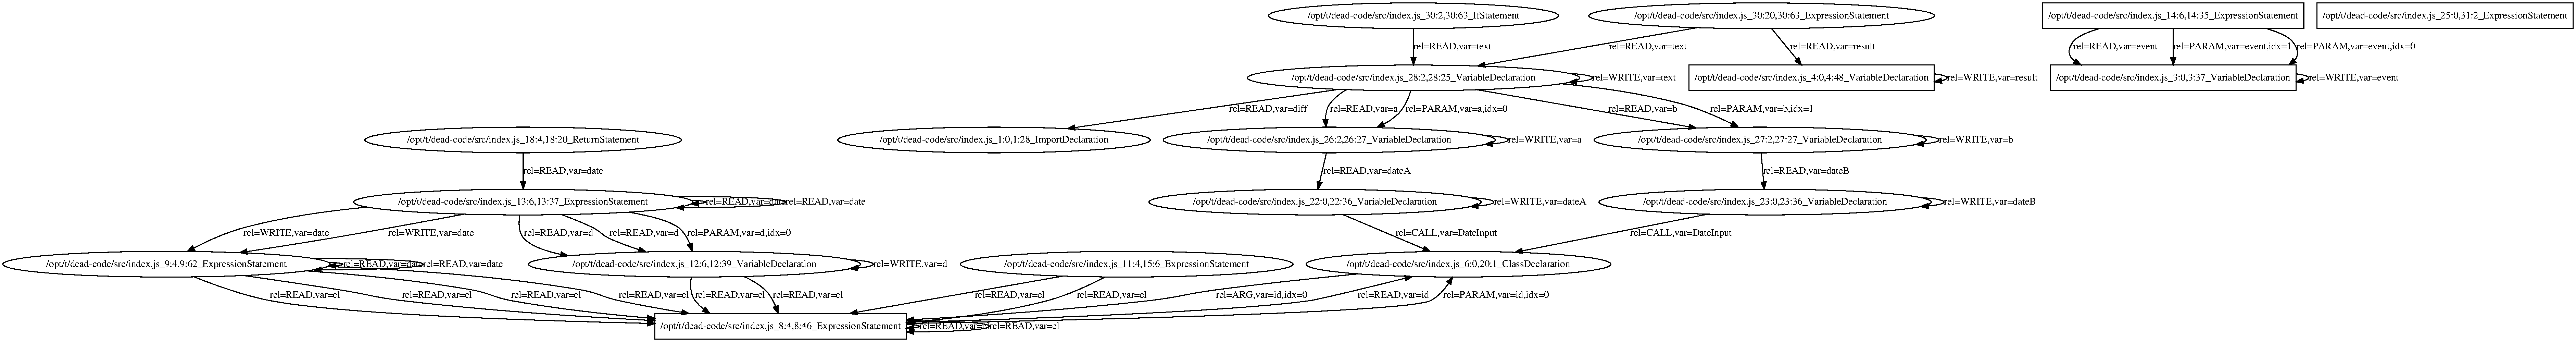
\includegraphics[width=\textwidth]{dead-code_graph_index.eps}
    \label{fig:deadcode}
   \caption{Example web application, index.js graph}
\end{figure}

As we can easily see in the graph, all nodes are connected to at least a terminal node. Therefore, we can intuitively say that the file does not contain dead code. We also know that at this moment of the analysis, all the dependencies are still considered dead code. The following file to analyse then would be the \texttt{diff.js} file of the project.

\begin{lstlisting}[language=Java, caption=\texttt{diff.js} file of the example web application]
import intervalToDuration from 'date-fns/intervalToDuration'
import formatDuration from 'date-fns/formatDuration'

function basicDiff(start, end) {
  return Math.abs(start - end)
}

export default function diff(start, end) {
  if (start && start instanceof Date && end && end instanceof Date)
    return formatDuration(intervalToDuration({ start, end }))
  else return null
}
\end{lstlisting}

The file, similarly to the previous one, starts with two imports (L1, L2) which import files from the library \texttt{date-fns}. After that, there are two functions defined in the file. The first one (L4-L6) is never exported, neither referenced anywhere else within this file. The second one (L8-L12), which is exported as default output of the module, has two parameters (L8). After checking if the parameters are defined and are date types (L9), it calculates the difference between both parameters using the functions imported at the beginning (L10). If the validation fails, it returns \texttt{null} (L11).

The file generates the following call graph. We can see that there are two sub graphs separated from each other. They represent the two different functions in the module. We know that the one that represents the second function (L8-L12) is linked by an export function to the \texttt{index.js} file (see page \pageref{fig:deadcode} for the full graph), while the other is effectively, dead code. We can also appreciate that the sub graph of the exported function contains a reference to the an import statement that references the \texttt{date-fns} library, which would mark it as "alive".

\begin{figure}[H]
  \centering
    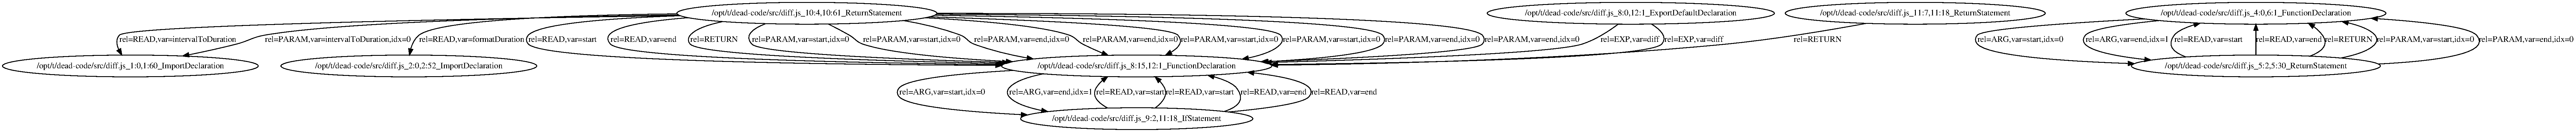
\includegraphics[width=\textwidth]{dead-code_graph_diff.eps}
    \label{fig:deadcode}
   \caption{Example web application, diff.js graph}
\end{figure}

The module does not import other modules, hence the remaining file, \texttt{old-diff.js} should be marked as dead. The remaining dependency, \texttt{dayjs}, should be marked as dead as well as it is not imported by any of the modules we have visited. The call graph generated by the remaining file and the edges between graph modules can be found in the full project graph in page \pageref{fig:deadcode}.

We introduce this project in the tool we created to verify if the output matches our expectations. As part of the configuration of the tool, we define \texttt{index.js} as the singe entry point of the application and exclude the folder in which the bundle will be created. The output of the tool for this project is the following. The output of the tool gives the following result.

\begin{verbatim}
  D E A D   C O D E
=> Dependencies 1 [ 'dayjs' ]
=> Modules 1 [ '/opt/t/dead-code/src/old-diff.js' ]
=> Statements 2 [
  '/opt/t/dead-code/src/diff.js_4:0,6:1_FunctionDeclaration',
  '/opt/t/dead-code/src/diff.js_5:2,5:30_ReturnStatement'
]
\end{verbatim}

The output matches the expected result. It marks one dependency as dead, \texttt{dayjs} and the file that is not imported, \texttt{old-diff.js}. It also correctly marks the function that we realised it is not used, which corresponds to the statements in the \texttt{diff.js} file in the lines 4 and 5.

\section{Chosen projects}

\subsection{\texttt{chalk}}
The project is composed of three files and two dependencies. The dependencies are two libraries named \texttt{ansi-styles} and \texttt{supports-color} that contain colour and terminal related utilities. The first one of the files is the longest and also the entry point of the library. It contains essentially all the logic behind it. The other two files, \texttt{template.js} and \texttt{util.js} are supporting functions for the main file like, for example, performing string substitutions or detect escape sequences. The project contains other files like types defintions for TypeScript, examples, unit tests or benchmarks.

The tool is configured to treat the project as a library. This means that the \texttt{Exports} statement nodes and the nodes that refer to \texttt{module.exports} assignments of the entry point are considered terminal nodes. The only entry point is the \texttt{index.js} file and the files related to test, benchmarks and examples have been excluded of the analysis. The call graph generated from this project can be fond on page \pageref{fig:chalk}.

The output of the tool for this project is the following:
\begin{verbatim}
  D E A D   C O D E
=> Dependencies 0 []
=> Modules 0 []
=> Statements 0 []
\end{verbatim}

This means that the tool was not able to detect any dead code within the project. This was our expectation based on the size of the project, its maturity and the community behind it.
\subsection{\texttt{Debug}}
The project is composed of four files and a single dependency named \texttt{ms} which provides function to transform amounts of milliseconds in different units of time. The entry point of the project is a file named \texttt{index.js}. This file is quite simple and essentially decided if it loads the version of the library for browsers (\texttt{browser.js}) or the version for Node.js (\texttt{node.js}). Independently of which version of the library is used, both files will import the \texttt{common.js} file which contains functions used in the implementation of both versions. There are other files like \texttt{test.js} or \texttt{karma.conf.js} which contain unit tests and their configuration, in addition of documentation and other files.

The tool is configured to treat the project as a library. The only entry point is the \texttt{index.js} file. Tests and other files are ignored. The output of the tool is the following:

\begin{verbatim}
  D E A D   C O D E
=> Dependencies 0 []
=> Modules 0 []
=> Statements 8 [
  '/opt/t/debug/src/browser.js_13:1,13:20_VariableDeclaration',
  '/opt/t/debug/src/browser.js_15:1,20:3_ReturnStatement',
  '/opt/t/debug/src/browser.js_16:2,19:3_IfStatement',
  '/opt/t/debug/src/browser.js_17:3,17:17_ExpressionStatement',
  '/opt/t/debug/src/browser.js_257:0,257:36_VariableDeclaration',
  '/opt/t/debug/src/browser.js_263:0,269:2_ExpressionStatement',
  '/opt/t/debug/src/browser.js_265:2,265:27_ReturnStatement',
  '/opt/t/debug/src/browser.js_267:2,267:56_ReturnStatement'
]
\end{verbatim}
In this case, the tool has marked some statements in the \texttt{browser.js} file as dead code. Those lines correspond to the two following snippets:

\begin{lstlisting}[language=Java, firstnumber=12, caption=First fragment of code of \texttt{browser.js} marked as dead code]
exports.destroy = (() => {
	let warned = false;

	return () => {
		if (!warned) {
			warned = true;
			console.warn('Instance method `debug.destroy()` is deprecated and no longer does anything.
			It will be removed in the next major version of `debug`.');
		}
	};
})();
\end{lstlisting}

\begin{lstlisting}[language=Java, firstnumber=255, caption=Second fragment of code of \texttt{browser.js} marked as dead code]
module.exports = require('./common')(exports);

const {formatters} = module.exports;

/**
 * Map %j to `JSON.stringify()`, since no Web Inspectors do that by default.
 */

formatters.j = function (v) {
	try {
		return JSON.stringify(v);
	} catch (error) {
		return '[UnexpectedJSONParseError]: ' + error.message;
	}
};
\end{lstlisting}

In the first case, we can see that those lines act as flag to ensure that the function is only executed once. We can see how in those lines a variable is declared, its value checked and then assigned a new value. Those three statements are not related with a terminal statement, and correctly they are marked as a dead code. However, intuitively we can see that these lines fulfil functionality and removing them will change the behaviour of the program, although it will not break it. Hence, this is not a problem of the dead code detection algorithm but a bug in  the call graph that is not able to detect the relationship between those statements. These lines are not marked in the \texttt{node.js} version because they do not exist.

The second case, we have some help from the comment in the code to understand what is happening. In L255, it imports the functions from the common library in the file \texttt{common.js}. As the comment indicates, for working in the browser's developer tools, one of the existing functions need to be modified. In L257 it extracts the object to modify, and in L256-260 it adds the functionality. In essence, it is modifying one property of an object created in a different file. Operations and changes happening at property level are one of the limitations of the algorithms described in this document, and a limitation in general to JavaScript static analysis. Those lines of codes reported, after understanding what they do, should be considered a false positive due to the limitations of the algorithms.

\section{General conclusions}
This method is able to provide more information about the location and potential dead code in a project to the user than industry linters by looking for patterns in the code and industry transpilers by performing tree shaking. Compared to linters, it is able to detect dead modules and dependencies, which is not possible as the analysis it performs is exclusive on a single file. Compared to transpilers performing tree shaking, it is able to detect individual statements within functions or classes that could be considered dead code, as the transpilers only discards functions and equivalent statements during the tree shaking process without analysing individual statements. The results it provides is something between both approaches that none of them is able to fully provide.

The experimental results show that the conceptual approach to detecting dead code in JavaScript is feasible. The algorithm described is easily understandable and conceptually simple, but effective. However, its results heavily depend on the quality of the call graph it uses. The call graph  design is also a fresh implementation based on new ideas different to the existing ones. The call graphs support modern features of JavaScript that existing tools did not support, as highlighted in \cite{metaCallGraphs}, and follows a different approach by associating nodes to statements in such a way that matches better our needs.

This is also the biggest issue with the current approach. The accuracy of the dead code detection algorithm depends on the call graph quality: the more relationships is able to find, the less amount of false positives it will find. As the call graph used in the proof of concept is a proof of concept as well, it cannot be considered "production ready" and there are patterns and relations that it is not able to detect.

The idiosyncrasy of the language makes it a huge challenge. Some of the short-comings of the language, like detecting the exact version of the language that is used or dealing with the dynamic nature of it makes static analysis a even bigger challenge. The fact that most of the tools use a dynamic or hybrid approach or aim to identify certain patterns in source files instead of a full project analysis is not a coincidence. It is also not a coincidence that most of the existing call-graphs algorithms and tool do not support ECMAScript 6. The amount of node types added in this version is almost as big as the total amount of the previous version. The increased complexity makes significantly harder to detect all the patters in the code that establish a relationship between the different statements.

Obtaining results on a simple project with a proof of concept implementation is possible, but the complexity of the implementation raises as soon as more language features are added, patterns used and the project growths. Even if we were targeting the latest stable version available at the moment, there are some language features like properties in objects are "dead" that are not possible as the granularity chose is not fine-grained enough.

\subsection{Output and lessons learnt}
The main output of this document is presenting a method to detect dead code in JavaScript projects of version 6 of ECMAScript. The research done and the experimental results prove that this method is at least worth considering when facing dead code in this type of projects.

There is a secondary output which is the tool used during the research for detecting dead code. This tool is proved during the research phase that, in its current state, is good enough for small projects but it soon gets out sized. As explained in the previous section, it is a proof of concept and it would require additional development effort to make it ready for use with general projects.

We learn that the basic ideas behind the algorithms explained, although conceptually simple, they are powerful and they could be applied possibly to other languages as far as a reasonable graph is created.

We faced several challenges related to JavaScript idiosyncrasies. We overcame some of them, like dealing with asynchronous code or the hoisting. However, other resulted to be much harder to overcome. Determining the version of ECMAScript running is still a challenge with complicated solutions, as features from different future versions can be used at the same time in a code base thanks to transpilation. Given a relatively modern JavaScript project, we know that it is can have features between ECMAScript 5 and the latest available at the moment without specifying exactly which version or features of the version.

We also learnt that objects and its dynamism is the biggest obstacle regarding static analysis of JavaScript. Objects are extremely dynamic, often changing their properties, types and values during runtime. These changes happen at expression level, which is the minimum granularity of composition, and they can be nested. We expected this to be a challenge and it proved to be. It is important to mention that we managed to mitigate part of this issue when the object part is a \texttt{this} expression, allow us to treat modern ES6 classes.

\subsection{Threads to validity}
The biggest thread to validity is the call graph used to apply the dead code detection algorithm. When the algorithm is not able to detect edges between the nodes it marks them as dead code. A bad quality call graph has less edges than a good quality call graph as it is able to identify less relationships between statements. Therefore, the algorithm tends to over report issues rather than under report them. In other words, the algorithm wrongly reports normal statements as dead rather than dead code statements as normal statements. The presence of dead code, as exposed in earlier chapters, do not "hurt" the functionality of a software, but the removal of "alive" code marked as dead code does.

The problem itself is not the algorithm described but the implementation. In the analysis in this document we have used a proof of concept of the call graph that is able to correctly detect most of the relationships between statements. However, there are many patterns that it is not able to identify and this becomes more obvious in bigger projects.

The results obtained are reproducible using the proof of concept of the algorithm implementation provided, but used in other projects can give a wide variety of results, specially when we need to take in consideration if other projects are targeting the concrete version of ECMAScript that the implementation and this document is considering. 

\subsection{Future work}
There are many opportunities of research in this area. The biggest improvement in the quality of the results is to detect more relationships between statements, or patterns that establish the existing relationships. The ever-growing specification of the language already sets an objective of keeping up implementations for the current relationships, but more could be added. The current proof of concept is a good start that highlights what is possible to do in this area, but the amount of features and cases makes it insufficient for dealing with many industry cases. It could be possible to even take a totally different approach building the call graph like in  \cite{MadsenMagnus2015Saoe} by using events in addition to statements to detect relationships between those in systems that make heavy use of event emitters and event listeners.

Going deeper in granularity is another option, as object properties are generally expressions and the current approach is not able to detect which ones are alive and which ones not. A deeper analysis of the Web API's and/or standard libraries available in the engine would allow a better classification of which functions of them lead to terminal nodes or not.

\appendix
\chapter{Project graphs}
\begin{figure}[htbp]
  \centering
    
\includegraphics[width=\textwidth]{dead-code_graph_project.pdf}
    \label{fig:deadcode}
   \caption{Example web application project graph}
\end{figure}
\begin{figure}[htbp]
    \centering
    \includegraphics[width=\textwidth]{chalk_graph_project.pdf}
    \label{fig:chalk}
\caption{\texttt{chalk} project graph}
\end{figure}
\begin{figure}[htbp]
    \centering
    \includegraphics[width=\textwidth]{debug_graph_project.pdf}
    \label{fig:debug}    
\caption{\texttt{debug} project graph}
\end{figure}

{
\bibliographystyle{alphaurl}
\bibliography{thesis}
}

\end{document}
